\documentclass[aspectratio=169]{beamer}

% ── Theme ────────────────────────────────────────────────────────────────────
\usetheme{Madrid}
\usecolortheme{whale}
\usefonttheme{professionalfonts}

% ── Packages ─────────────────────────────────────────────────────────────────
\usepackage[utf8]{inputenc}
\usepackage[T1]{fontenc}
\usepackage[english]{babel}
\usepackage{graphicx}
\usepackage{booktabs}
\usepackage{amsmath}
\usepackage{amssymb}
\usepackage{xcolor}
\usepackage{tikz}
\usetikzlibrary{shapes,arrows.meta,positioning}
\usepackage{listings}
\usepackage{multicol}

\graphicspath{{images/}}

% ── Colors ───────────────────────────────────────────────────────────────────
\definecolor{univ}{RGB}{0,70,127}
\definecolor{accent}{RGB}{220,80,30}
\definecolor{lightgray}{RGB}{245,245,245}

\setbeamercolor{frametitle}{bg=univ,fg=white}
\setbeamercolor{title}{fg=white}
\setbeamercolor{author}{fg=white}
\setbeamercolor{institute}{fg=white!85}
\setbeamercolor{date}{fg=white!85}
\setbeamercolor{block title}{bg=univ!90,fg=white}
\setbeamercolor{block body}{bg=univ!8}
\setbeamercolor{alerted text}{fg=accent}
\setbeamercolor{structure}{fg=univ}

% ── Remove nav symbols ───────────────────────────────────────────────────────
\setbeamertemplate{navigation symbols}{}
\setbeamertemplate{footline}[frame number]

% ── Listings style ───────────────────────────────────────────────────────────
\lstset{basicstyle=\ttfamily\tiny, breaklines=true, frame=single,
        backgroundcolor=\color{lightgray}}

% ════════════════════════════════════════════════════════════════════════════
\title[ExamGen]{\textbf{ExamGen}\\
  \large AI-Powered Intelligent Exam Generation Platform}
\subtitle{End-of-Study Project Defense}
\author[Biskra 2026]{Student Team}
\institute[Univ.\ Biskra]{
  Department of Computer Science\\
  University of Mohamed Khider Biskra\\[4pt]
  \textit{Supervisor: Dr.\ Laid KAHLOUL}
}
\date{Academic Year 2025--2026}
% ════════════════════════════════════════════════════════════════════════════

\begin{document}

% ── Title Slide ──────────────────────────────────────────────────────────────
\begin{frame}[plain]
  \begin{tikzpicture}[remember picture, overlay]
    \fill[univ] (current page.north west) rectangle (current page.south east);
    \node[opacity=0.08] at (current page.center) {%
      \fontsize{120}{120}\selectfont\bfseries EG};
  \end{tikzpicture}
  \titlepage
\end{frame}

% ── Table of Contents ────────────────────────────────────────────────────────
\begin{frame}{Outline}
  \tableofcontents
\end{frame}

% ════════════════════════════════════════════════════════════════════════════
\section{Introduction}
% ════════════════════════════════════════════════════════════════════════════

\begin{frame}{Background and Motivation}
  \begin{columns}[T]
    \begin{column}{0.55\textwidth}
      \textbf{The Problem}
      \begin{itemize}
        \item Constructing university exams is cognitively demanding
        \item Must satisfy: pedagogical objectives, Bloom's levels,
              linguistic consistency, avoid repeating past questions
        \item Algerian universities face a \alert{bilingual PDF archive}
              (French + Arabic) with no machine-readable indexing
      \end{itemize}
      \vspace{6pt}
      \textbf{The Gap}
      \begin{itemize}
        \item No existing system handles bilingual IDP +
              language-aware RAG + independent quality evaluation
      \end{itemize}
    \end{column}
    \begin{column}{0.42\textwidth}
      \begin{block}{Our Solution}
        \textbf{ExamGen} — an AI-powered exam generation
        platform that assists teachers by automatically
        producing high-quality, pedagogically calibrated
        questions from their own course materials.\\[6pt]
        \textit{The AI acts as a decision-support tool;
        instructors review, edit, and validate all output.}
      \end{block}
    \end{column}
  \end{columns}
\end{frame}

\begin{frame}{Thesis Statement and Key Results}
  \begin{block}{Thesis}
    A \textbf{bilingual, schema-enforced, RAG-augmented pipeline} --- combining
    intelligent document processing, language-aware hybrid retrieval, and an
    independent post-generation quality evaluator --- can produce factually grounded,
    cognitively calibrated examination questions \emph{without model fine-tuning}.
  \end{block}

  \vspace{8pt}
  \begin{columns}[T]
    \begin{column}{0.32\textwidth}
      \centering
      {\Large\bfseries\color{accent} 87.5\%}\\[2pt]
      Factual Accuracy
    \end{column}
    \begin{column}{0.32\textwidth}
      \centering
      {\Large\bfseries\color{accent} 83.8\%}\\[2pt]
      Retrieval Effectiveness
    \end{column}
    \begin{column}{0.32\textwidth}
      \centering
      {\Large\bfseries\color{accent} 704}\\[2pt]
      Bloom-labelled Questions
    \end{column}
  \end{columns}

  \vspace{8pt}
  \centering
  \textit{Evaluated on 137 real bilingual university documents across 5 subjects}
\end{frame}

% ════════════════════════════════════════════════════════════════════════════
\section{State of the Art}
% ════════════════════════════════════════════════════════════════════════════

\begin{frame}{Related Work: Key Reference Studies}
  \begin{tabular}{lp{7.5cm}}
    \toprule
    \textbf{Study} & \textbf{Key Contribution Adopted in ExamGen} \\
    \midrule
    Mucciaccia et al.\ (2025) &
      Schema-enforced generation + automated LLM-as-judge review \\[4pt]
    Isley et al.\ (2025) &
      RAG grounding; post-generation evaluator; iterative refinement
      (91 courses, $\approx$1,700 students) \\[4pt]
    Morris et al.\ (2024) &
      \textit{Answer extractability} as primary quality metric;
      SAQ grading rubrics \\[4pt]
    Meissner et al.\ (2024) &
      Independent Bloom classifier (do not trust generator's self-reported level) \\
    \bottomrule
  \end{tabular}
\end{frame}

\begin{frame}{Positioning of ExamGen}
  \centering
  \begin{tabular}{lcccc}
    \toprule
    \textbf{Feature} & \textbf{Mucciaccia'25} & \textbf{Isley'25}
      & \textbf{Morris'24} & \textbf{ExamGen} \\
    \midrule
    Bilingual corpus          & $\times$ & $\times$ & $\times$ & \checkmark \\
    IDP pipeline (5 stages)   & partial  & $\times$ & $\times$ & \checkmark \\
    VLM diagram transcription & $\times$ & $\times$ & $\times$ & \checkmark \\
    Language-aware hybrid RAG & $\times$ & \checkmark & \checkmark & \checkmark \\
    Schema-enforced generation & \checkmark & \checkmark & $\times$ & \checkmark \\
    Independent Bloom classifier & $\times$ & $\times$ & $\times$ & \checkmark \\
    Post-generation evaluator & \checkmark & \checkmark & $\times$ & \checkmark \\
    Multi-tenant web app      & $\times$ & $\times$ & $\times$ & \checkmark \\
    \bottomrule
  \end{tabular}

  \vspace{6pt}
  \alert{No existing system simultaneously addresses all four requirements.}
\end{frame}

% ════════════════════════════════════════════════════════════════════════════
\section{System Architecture}
% ════════════════════════════════════════════════════════════════════════════

\begin{frame}{Iterative Development: Three Prototype Failures}
  ExamGen evolved through three versions. V2 revealed three concrete failures:

  \vspace{6pt}
  \begin{block}{F1 — No structured output}
    Free-text instead of JSON; regex parsing failed on $\approx$30\% of responses.\\
    \textbf{Fix:} \texttt{instructor} library with self-healing Pydantic schema (max\_retries=3)
  \end{block}

  \begin{block}{F2 — Free-tier model fidelity}
    Models ignored structural constraints (e.g.\ ``exactly 4 choices'').\\
    \textbf{Fix:} Switch to DeepSeek-V4-Flash with fallback chain (Gemini $\to$ Claude)
  \end{block}

  \begin{block}{F3 — Semantic retrieval blends topics}
    Retrieved passages mixed subjects and years, diluting instructor style.\\
    \textbf{Fix:} Separate \textbf{style anchors} from \textbf{RAG factual context}
    in two distinct prompt blocks
  \end{block}
\end{frame}

\begin{frame}{Four-Layer Architecture}
  \centering
  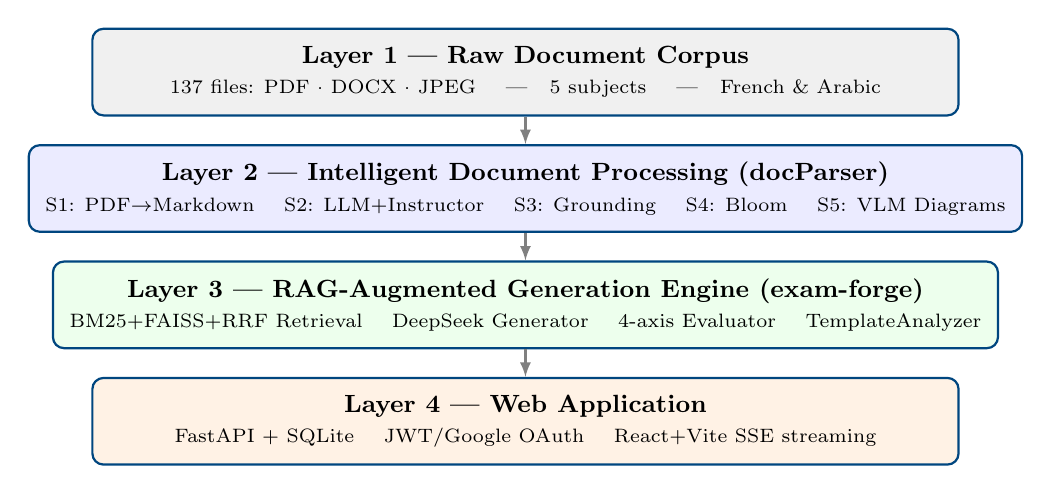
\begin{tikzpicture}[font=\small, node distance=0.4cm]
    \tikzstyle{layer}=[draw=univ, thick, rounded corners=4pt,
      minimum width=11cm, minimum height=1.1cm, align=center, inner sep=6pt]
    \tikzstyle{arrow}=[->, >=latex, thick, gray]

    \node[layer, fill=gray!12] (L1)
      {\textbf{Layer 1 — Raw Document Corpus}\\
       \scriptsize 137 files: PDF · DOCX · JPEG \quad|\quad 5 subjects \quad|\quad French \& Arabic};

    \node[layer, fill=blue!8, below=0.35cm of L1] (L2)
      {\textbf{Layer 2 — Intelligent Document Processing (docParser)}\\
       \scriptsize S1: PDF$\to$Markdown \quad S2: LLM+Instructor \quad S3: Grounding
       \quad S4: Bloom \quad S5: VLM Diagrams};

    \node[layer, fill=green!7, below=0.35cm of L2] (L3)
      {\textbf{Layer 3 — RAG-Augmented Generation Engine (exam-forge)}\\
       \scriptsize BM25+FAISS+RRF Retrieval \quad DeepSeek Generator
       \quad 4-axis Evaluator \quad TemplateAnalyzer};

    \node[layer, fill=orange!10, below=0.35cm of L3] (L4)
      {\textbf{Layer 4 — Web Application}\\
       \scriptsize FastAPI + SQLite \quad JWT/Google OAuth \quad React+Vite SSE streaming};

    \draw[arrow] (L1) -- (L2);
    \draw[arrow] (L2) -- (L3);
    \draw[arrow] (L3) -- (L4);
  \end{tikzpicture}
\end{frame}

% ════════════════════════════════════════════════════════════════════════════
\section{Implementation}
% ════════════════════════════════════════════════════════════════════════════

\begin{frame}{Dataset}
  \centering
  \begin{tabular}{lrrrrr}
    \toprule
    \textbf{Subject} & \textbf{Raw files} & \textbf{JSON files}
      & \textbf{Exercises} & \textbf{Questions} & \textbf{Lang.} \\
    \midrule
    Algorithms     & 36  & 25  & 71  & 195 & French \\
    Software Eng.  & 30  & 22  & 58  & 175 & French \\
    Compilation    & 28  & 20  & 62  & 210 & French \\
    Commerce       & 14  &  8  & 24  &  58 & Arabic \\
    Law            & 29  & 11  & 26  &  66 & Arabic \\
    \midrule
    \textbf{Total} & \textbf{137} & \textbf{86} & \textbf{241} & \textbf{704} & Fr./Ar. \\
    \bottomrule
  \end{tabular}

  \vspace{8pt}
  \begin{columns}[T]
    \begin{column}{0.48\textwidth}
      \textbf{Hardware:} Intel Core i7-10750H, 16 GB RAM, Ubuntu 22.04 (WSL2)
    \end{column}
    \begin{column}{0.48\textwidth}
      \textbf{Stack:} Python 3.12, Docling, PyMuPDF, FAISS-CPU, FastAPI, React+Vite
    \end{column}
  \end{columns}
\end{frame}

\begin{frame}{docParser: 5-Stage IDP Pipeline}
  \begin{enumerate}
    \item \textbf{Stage 1 — PDF $\to$ Markdown}\\
          Docling with TableFormer (table structure) + RTL-safe export.
          PyMuPDF hybrid fill for formula/pseudocode recovery.

    \vspace{4pt}
    \item \textbf{Stage 2 — LLM Extraction with Self-Healing Schema}\\
          \texttt{instructor} intercepts Pydantic errors $\to$ correction prompts
          (max\_retries=3). Schema: Exam $\supset$ Exercise $\supset$ Question.

    \vspace{4pt}
    \item \textbf{Stage 3 — Grounding Validation}\\
          Confidence score $c = \max(0,\;1 - 0.15|\mathcal{W}|
          - 0.5\cdot\mathbf{1}[\mathcal{E}{=}\varnothing] - \ldots)$.
          Flag if $c < 0.70$.

    \vspace{4pt}
    \item \textbf{Stage 4 — Bloom Classification}\\
          Independent classifier (\texttt{gpt-oss-120b}, temp=0):
          Factual / Conceptual / Procedural / Metacognitive.

    \vspace{4pt}
    \item \textbf{Stage 5 — VLM Diagram Transcription}\\
          Qwen2.5-VL-72B (primary) or Gemini-2.0-Flash (fallback);
          linked to nearest preceding question.
  \end{enumerate}
\end{frame}

\begin{frame}{Hybrid RAG: Language-Aware Retrieval}
  \begin{columns}[T]
    \begin{column}{0.52\textwidth}
      \textbf{HybridRetrieve$(q, \text{subj}, k{=}10)$}
      \begin{enumerate}
        \item Compute arabic\_ratio$(q)$
        \item \textbf{Sparse:} BM25 top-$k$ (exact term matching)
        \item \textbf{Dense:}
          \begin{itemize}
            \item Arabic ratio $> 0.15$ $\Rightarrow$ \textbf{AraBERT} + FAISS
            \item Otherwise $\Rightarrow$ \textbf{MiniLM} (multilingual)
          \end{itemize}
        \item \textbf{Fusion:} RRF$(d) = \sum_r \frac{1}{60 + \text{rank}_r(d)}$
        \item Cap at 2 chunks per source file
      \end{enumerate}

      \vspace{6pt}
      \textbf{Cloud:} Supabase + pgvector\\
      (scoped by user\_id + subject)
    \end{column}
    \begin{column}{0.44\textwidth}
      \begin{block}{Key Design: Style Separation}
        Two distinct prompt blocks prevent topic blending (F3):
        \begin{itemize}
          \item \textbf{[STYLE ANCHORS]} — 3--6 few-shot examples
                filtered by subject + Bloom level
          \item \textbf{[COURSE MATERIAL - RAG]} — retrieved chunks
        \end{itemize}
      \end{block}

      \vspace{6pt}
      \begin{block}{4-Axis Evaluator}
        \begin{enumerate}
          \item \texttt{factual\_ok}
          \item \texttt{level\_correct}
          \item \texttt{quality}: good / needs\_revision / reject
          \item \texttt{difficulty\_fair}
        \end{enumerate}
      \end{block}
    \end{column}
  \end{columns}
\end{frame}

% ════════════════════════════════════════════════════════════════════════════
\section{Web Interface}
% ════════════════════════════════════════════════════════════════════════════

\begin{frame}{Web Application Overview}
  \begin{columns}[T]
    \begin{column}{0.48\textwidth}
      \centering
      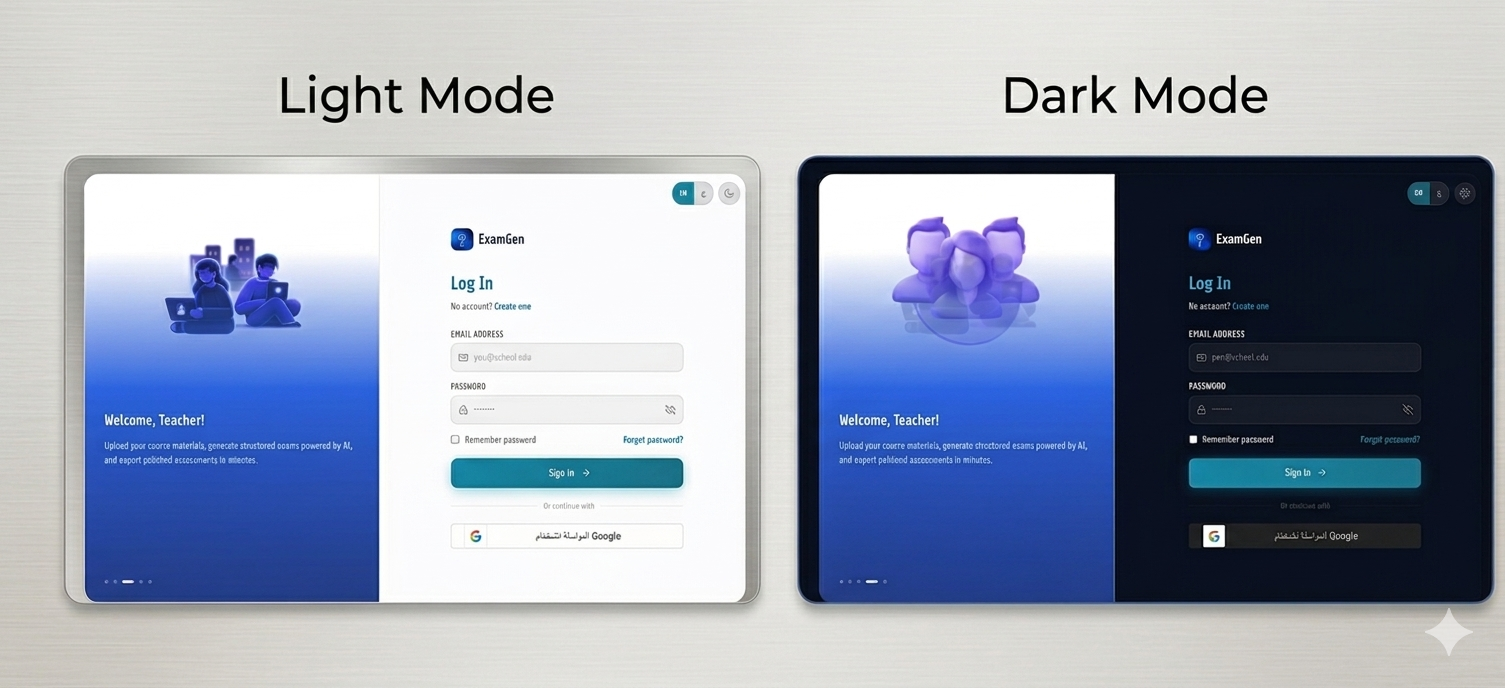
\includegraphics[width=\linewidth]{images/web_login.png}\\
      \small Login (email / Google OAuth 2.0)
    \end{column}
    \begin{column}{0.48\textwidth}
      \centering
      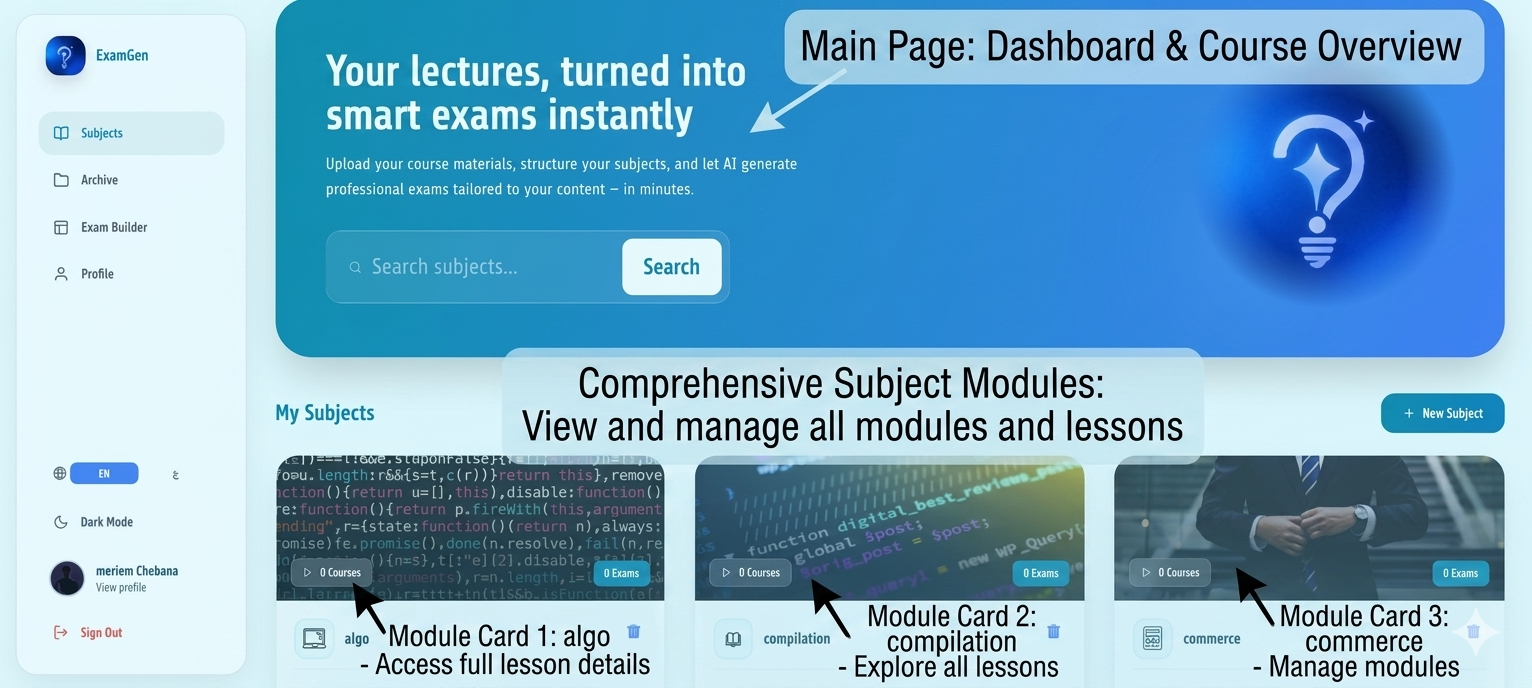
\includegraphics[width=\linewidth]{images/web_dashboard.png}\\
      \small Subject dashboard
    \end{column}
  \end{columns}
\end{frame}

\begin{frame}{Exam Generation Workflow}
  \centering
  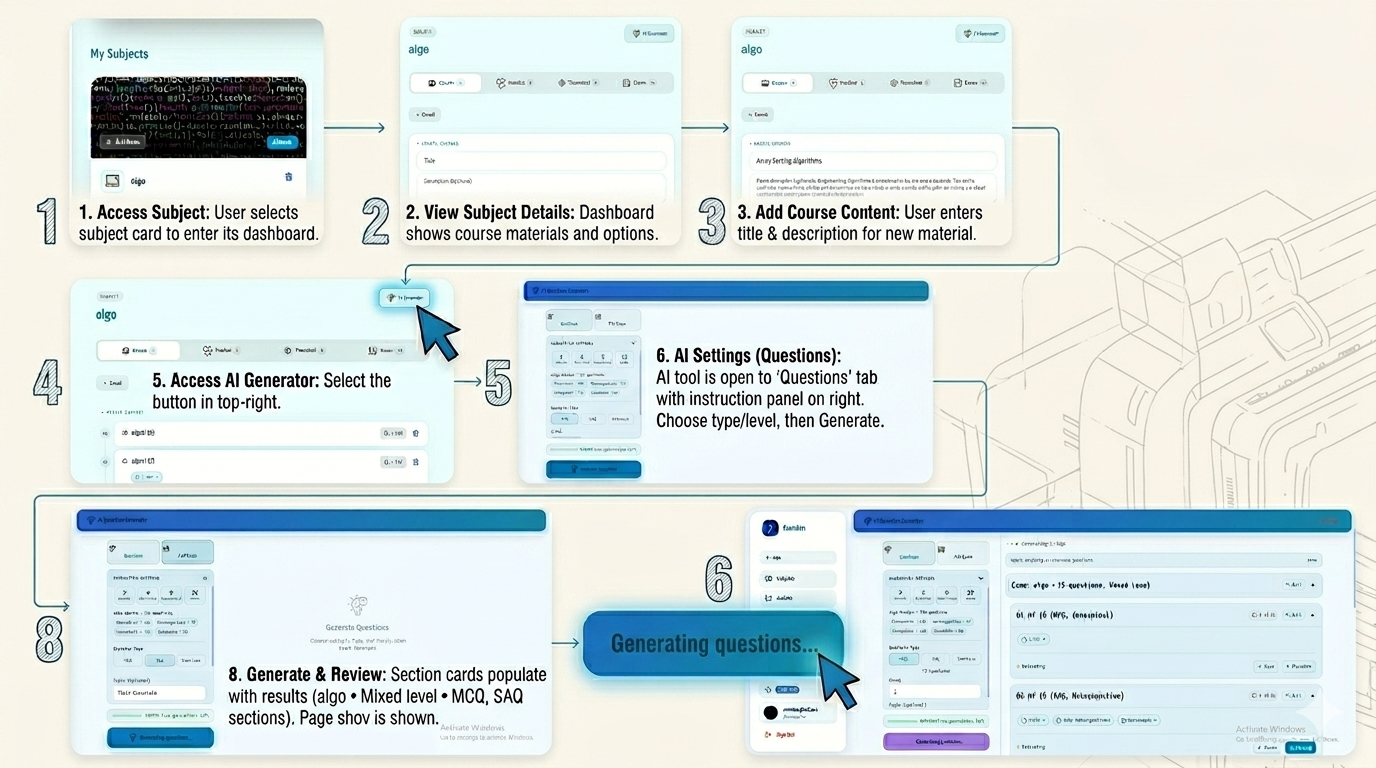
\includegraphics[width=\textwidth, height=6.5cm, keepaspectratio]{images/web_generation.png}

  \vspace{4pt}
  \small
  Select subject $\to$ configure type (MCQ/SAQ/Exercise) + Bloom level
  $\to$ questions stream \textbf{card-by-card via SSE} $\to$ accept / edit / reject
\end{frame}

\begin{frame}{Archive and Exam Builder}
  \begin{columns}[T]
    \begin{column}{0.48\textwidth}
      \centering
      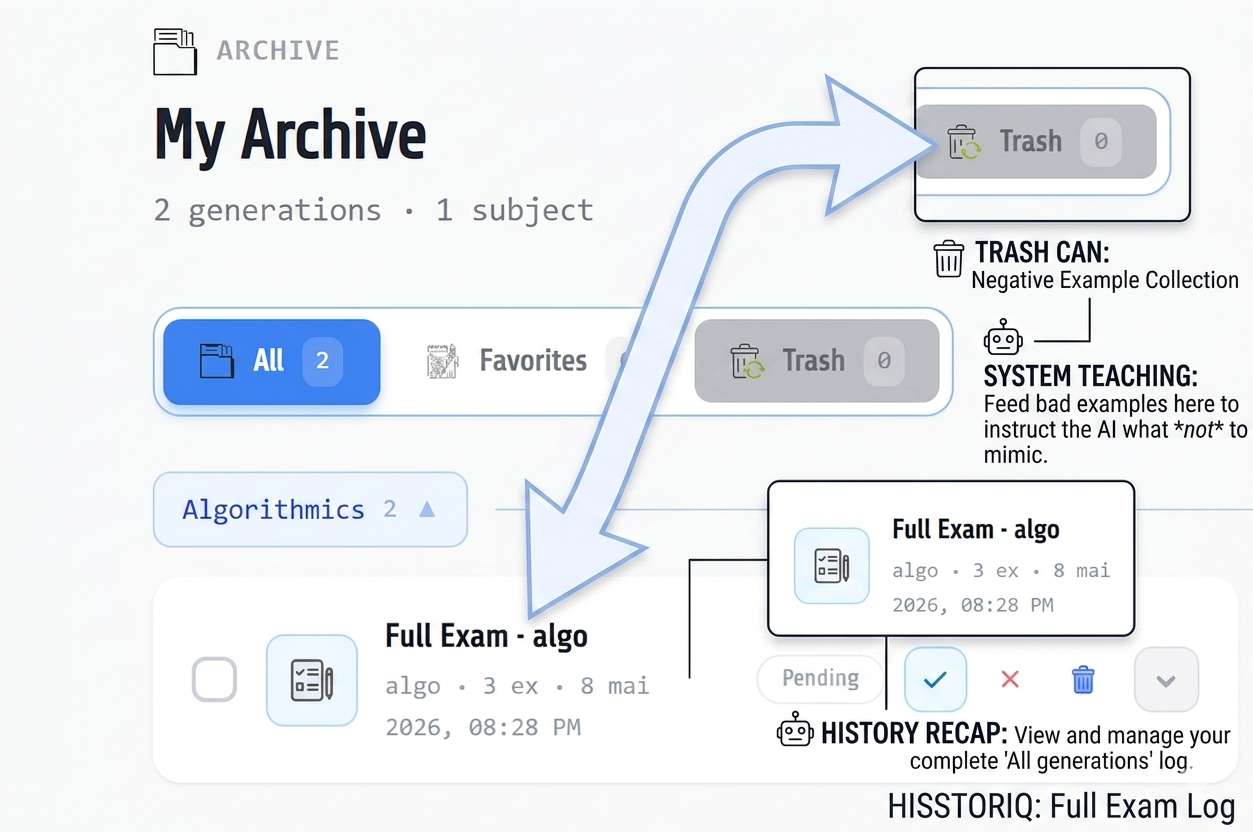
\includegraphics[width=\linewidth]{images/web_archive.png}\\
      \small Exam archive (browsable history)
    \end{column}
    \begin{column}{0.48\textwidth}
      \centering
      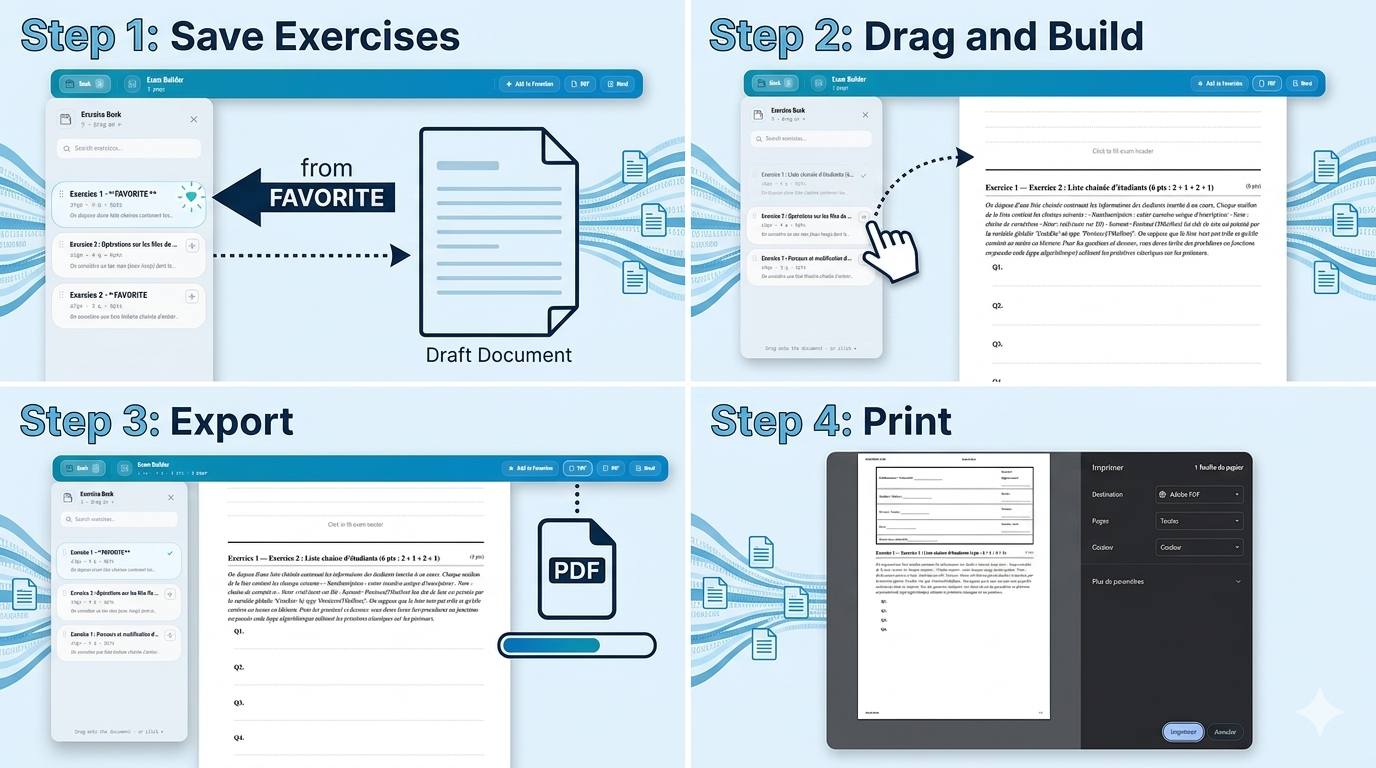
\includegraphics[width=\linewidth]{images/web_builder.png}\\
      \small Exam builder (assemble \& export)
    \end{column}
  \end{columns}
\end{frame}

% ════════════════════════════════════════════════════════════════════════════
\section{Results and Evaluation}
% ════════════════════════════════════════════════════════════════════════════

\begin{frame}{docParser Processing Results (137 documents)}
  \centering
  \begin{tabular}{lrr}
    \toprule
    \textbf{Metric} & \textbf{Count} & \textbf{Proportion} \\
    \midrule
    Successful Docling conversion       & 124 & 90.5\% \\
    PyMuPDF fallback used               &  13 &  9.5\% \\
    Hybrid formula/code fill triggered  &  41 & 33.1\% \\
    \midrule
    \textbf{Accepted} ($c \geq 0.70$)   &  86 & \textbf{62.8\%} \\
    Flagged for review ($c < 0.70$)     &  18 & 13.1\% \\
    Rejected (no extractable questions) &  33 & 24.1\% \\
    \midrule
    Visual diagrams extracted (Stage 5) &  47 & --- \\
    \quad Described by Qwen2.5-VL-72B   &  42 & 89.4\% \\
    \quad Described by Gemini-2.0-Flash &   5 & 10.6\% \\
    \bottomrule
  \end{tabular}

  \vspace{4pt}
  \small Of 33 rejected: 21 answer-key sheets (no question text) +
         12 low-resolution scans.
\end{frame}

\begin{frame}{Generation Quality (120 sampled questions)}
  \centering
  \begin{tabular}{lrrrr}
    \toprule
    \textbf{Subject} & \textbf{factual\_ok} & \textbf{level\_correct}
      & \textbf{quality: good} & \textbf{diff.\ fair} \\
    \midrule
    Algorithms    & 87.5\% & 79.2\% & 75.0\% & 83.3\% \\
    Software Eng. & 91.7\% & 83.3\% & 83.3\% & 87.5\% \\
    Compilation   & 87.5\% & 83.3\% & 79.2\% & 83.3\% \\
    Commerce      & 87.5\% & 79.2\% & 79.2\% & 87.5\% \\
    Law           & 83.3\% & 75.0\% & 70.8\% & 79.2\% \\
    \midrule
    \textbf{Overall} & \textbf{87.5\%} & \textbf{79.2\%}
      & \textbf{77.5\%} & \textbf{84.2\%} \\
    \bottomrule
  \end{tabular}

  \vspace{6pt}
  \begin{columns}[T]
    \begin{column}{0.48\textwidth}
      \small 87.5\% factual accuracy $\approx$ upper range reported by Mucciaccia et al.
    \end{column}
    \begin{column}{0.48\textwidth}
      \small Law scores lowest: small Arabic corpus (66 questions, 11 JSON files)
    \end{column}
  \end{columns}
\end{frame}

\begin{frame}{Retrieval Effectiveness (50 held-out queries)}
  \centering
  \begin{tabular}{lccc}
    \toprule
    \textbf{Configuration} & \textbf{French subjects}
      & \textbf{Arabic (Law)} & \textbf{Overall} \\
    \midrule
    BM25 only                              & 79.0\% & 62.0\% & 74.0\% \\
    Dense only (multilingual MiniLM)       & 81.0\% & 68.0\% & 77.2\% \\
    Dense only (AraBERT for Law)           & 83.0\% & 81.0\% & 82.6\% \\
    BM25 + MiniLM (RRF, no routing)       & 84.0\% & 71.0\% & 80.8\% \\
    \textbf{BM25 + AraBERT/MiniLM (RRF + routing)}
      & \textbf{85.0\%} & \textbf{81.0\%} & \textbf{83.8\%} \\
    \bottomrule
  \end{tabular}

  \vspace{8pt}
  \alert{Language-aware routing to AraBERT: +10 points on Arabic queries}\\
  \small (81.0\% vs.\ 71.0\% — confirms necessity of dedicated Arabic embeddings)
\end{frame}

% ════════════════════════════════════════════════════════════════════════════
\section{Conclusion}
% ════════════════════════════════════════════════════════════════════════════

\begin{frame}{Summary of Contributions}
  \begin{enumerate}
    \item \textbf{Bilingual IDP (docParser)}\\
          5-stage pipeline: 90.5\% conversion success, 704 Bloom-labelled questions,
          89.4\% VLM diagram description by Qwen2.5-VL

    \vspace{4pt}
    \item \textbf{Language-aware hybrid RAG}\\
          AraBERT routing + BM25 + RRF $\Rightarrow$ \textbf{83.8\%} retrieval effectiveness,
          +10 pts on Arabic queries

    \vspace{4pt}
    \item \textbf{Schema-enforced generation}\\
          \texttt{instructor} + dual-prompt architecture $\Rightarrow$ \textbf{87.5\%} factual accuracy

    \vspace{4pt}
    \item \textbf{Independent quality evaluation}\\
          4-axis evaluator confirms 79.2\% Bloom-level accuracy;
          motivates independent Stage-4 classifier

    \vspace{4pt}
    \item \textbf{Multi-tenant web platform}\\
          React + FastAPI + SSE real-time streaming; JWT + Google OAuth 2.0
  \end{enumerate}
\end{frame}

\begin{frame}{Limitations and Future Work}
  \begin{columns}[T]
    \begin{column}{0.48\textwidth}
      \textbf{Current Limitations}
      \begin{itemize}
        \item Law corpus sparsity (66 questions) $\to$ lowest scores
        \item No human-labelled ground truth; LLM evaluator is upper-bound estimate
        \item API dependency (DeepSeek, Gemini, GPT-OSS) $\to$ cloud required
        \item 12 low-resolution PDFs rejected (no OCR)
      \end{itemize}
    \end{column}
    \begin{column}{0.48\textwidth}
      \textbf{Future Directions}
      \begin{enumerate}
        \item \textbf{Unconditional OCR} (Tesseract/PaddleOCR) for low-res scans
        \item \textbf{IRT-based psychometric validation} via real exam deployments
        \item \textbf{On-device fine-tuned model} (Qwen2.5-7B or Mistral-7B)
              for offline operation and API independence
      \end{enumerate}
    \end{column}
  \end{columns}
\end{frame}

% ── Thank You ────────────────────────────────────────────────────────────────
\begin{frame}[plain]
  \begin{tikzpicture}[remember picture, overlay]
    \fill[univ] (current page.north west) rectangle (current page.south east);
  \end{tikzpicture}
  \begin{center}
    \vspace{1.5cm}
    {\color{white}\Large\bfseries Thank You}\\[12pt]
    {\color{white!80}\large Questions?}\\[20pt]
    \color{white!70}
    \textit{We sincerely thank our supervisor, Dr.\ Laid KAHLOUL,}\\
    \textit{and Ms.\ Nour El Houda Ben Chaabene for their guidance.}\\[4pt]
    \textit{Special thanks to Al Abbas Abbara for his kind support.}
  \end{center}
\end{frame}

\end{document}
